\subsection{(W) Maneuverability Uncertainty Intersection}\label{s:uncertaintyIntersection}
    \noindent Prediction of \emph{impact area} based on intruder position/velocity/estimated maneuverability, usable for \emph{expected adversarial behaviour}. Intersection polytope volume calculation \cite{lawrence1991polytope}
    
    \begin{figure}[H]
    	\centering
        \begin{subfigure}{0.48\textwidth}
            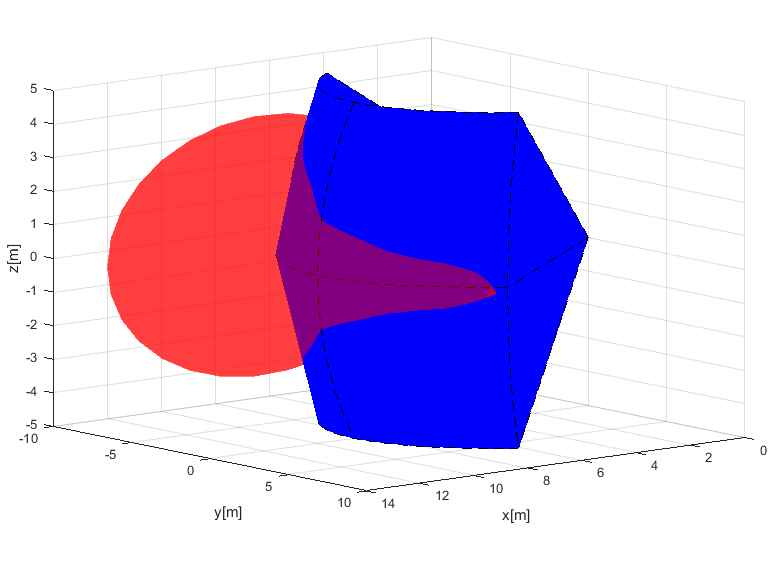
\includegraphics[width=0.9\linewidth]{\FIGDIR/TE013ElipticConeIntersecitonExample}
            \caption{\emph{Avoidance Grid} Intersection.}
            \label{fig:ellipticConeIntersectionExample}
        \end{subfigure}
        \begin{subfigure}{0.48\textwidth}
            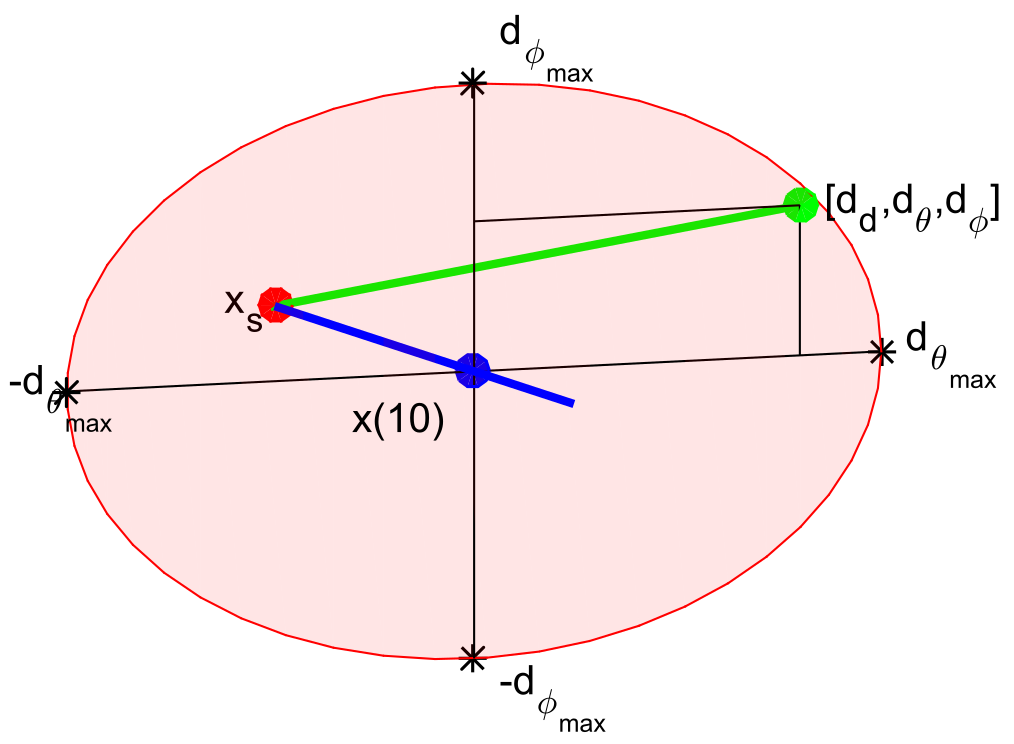
\includegraphics[width=0.9\linewidth]{\FIGDIR/TE014ElipticConeIOnePoint} 
            \caption{Horizontal slice.}
            \label{fig:ellipticalConeHorizontalSlice}
        \end{subfigure}
        \caption{Elliptical cone represented maneuverability approximation. }
        \label{fig:ellipticalConeRepresentedManuevurabilityApproximation}
    \end{figure}
    
    \begin{figure}[H]
    	\centering
        \begin{subfigure}{0.48\textwidth}
            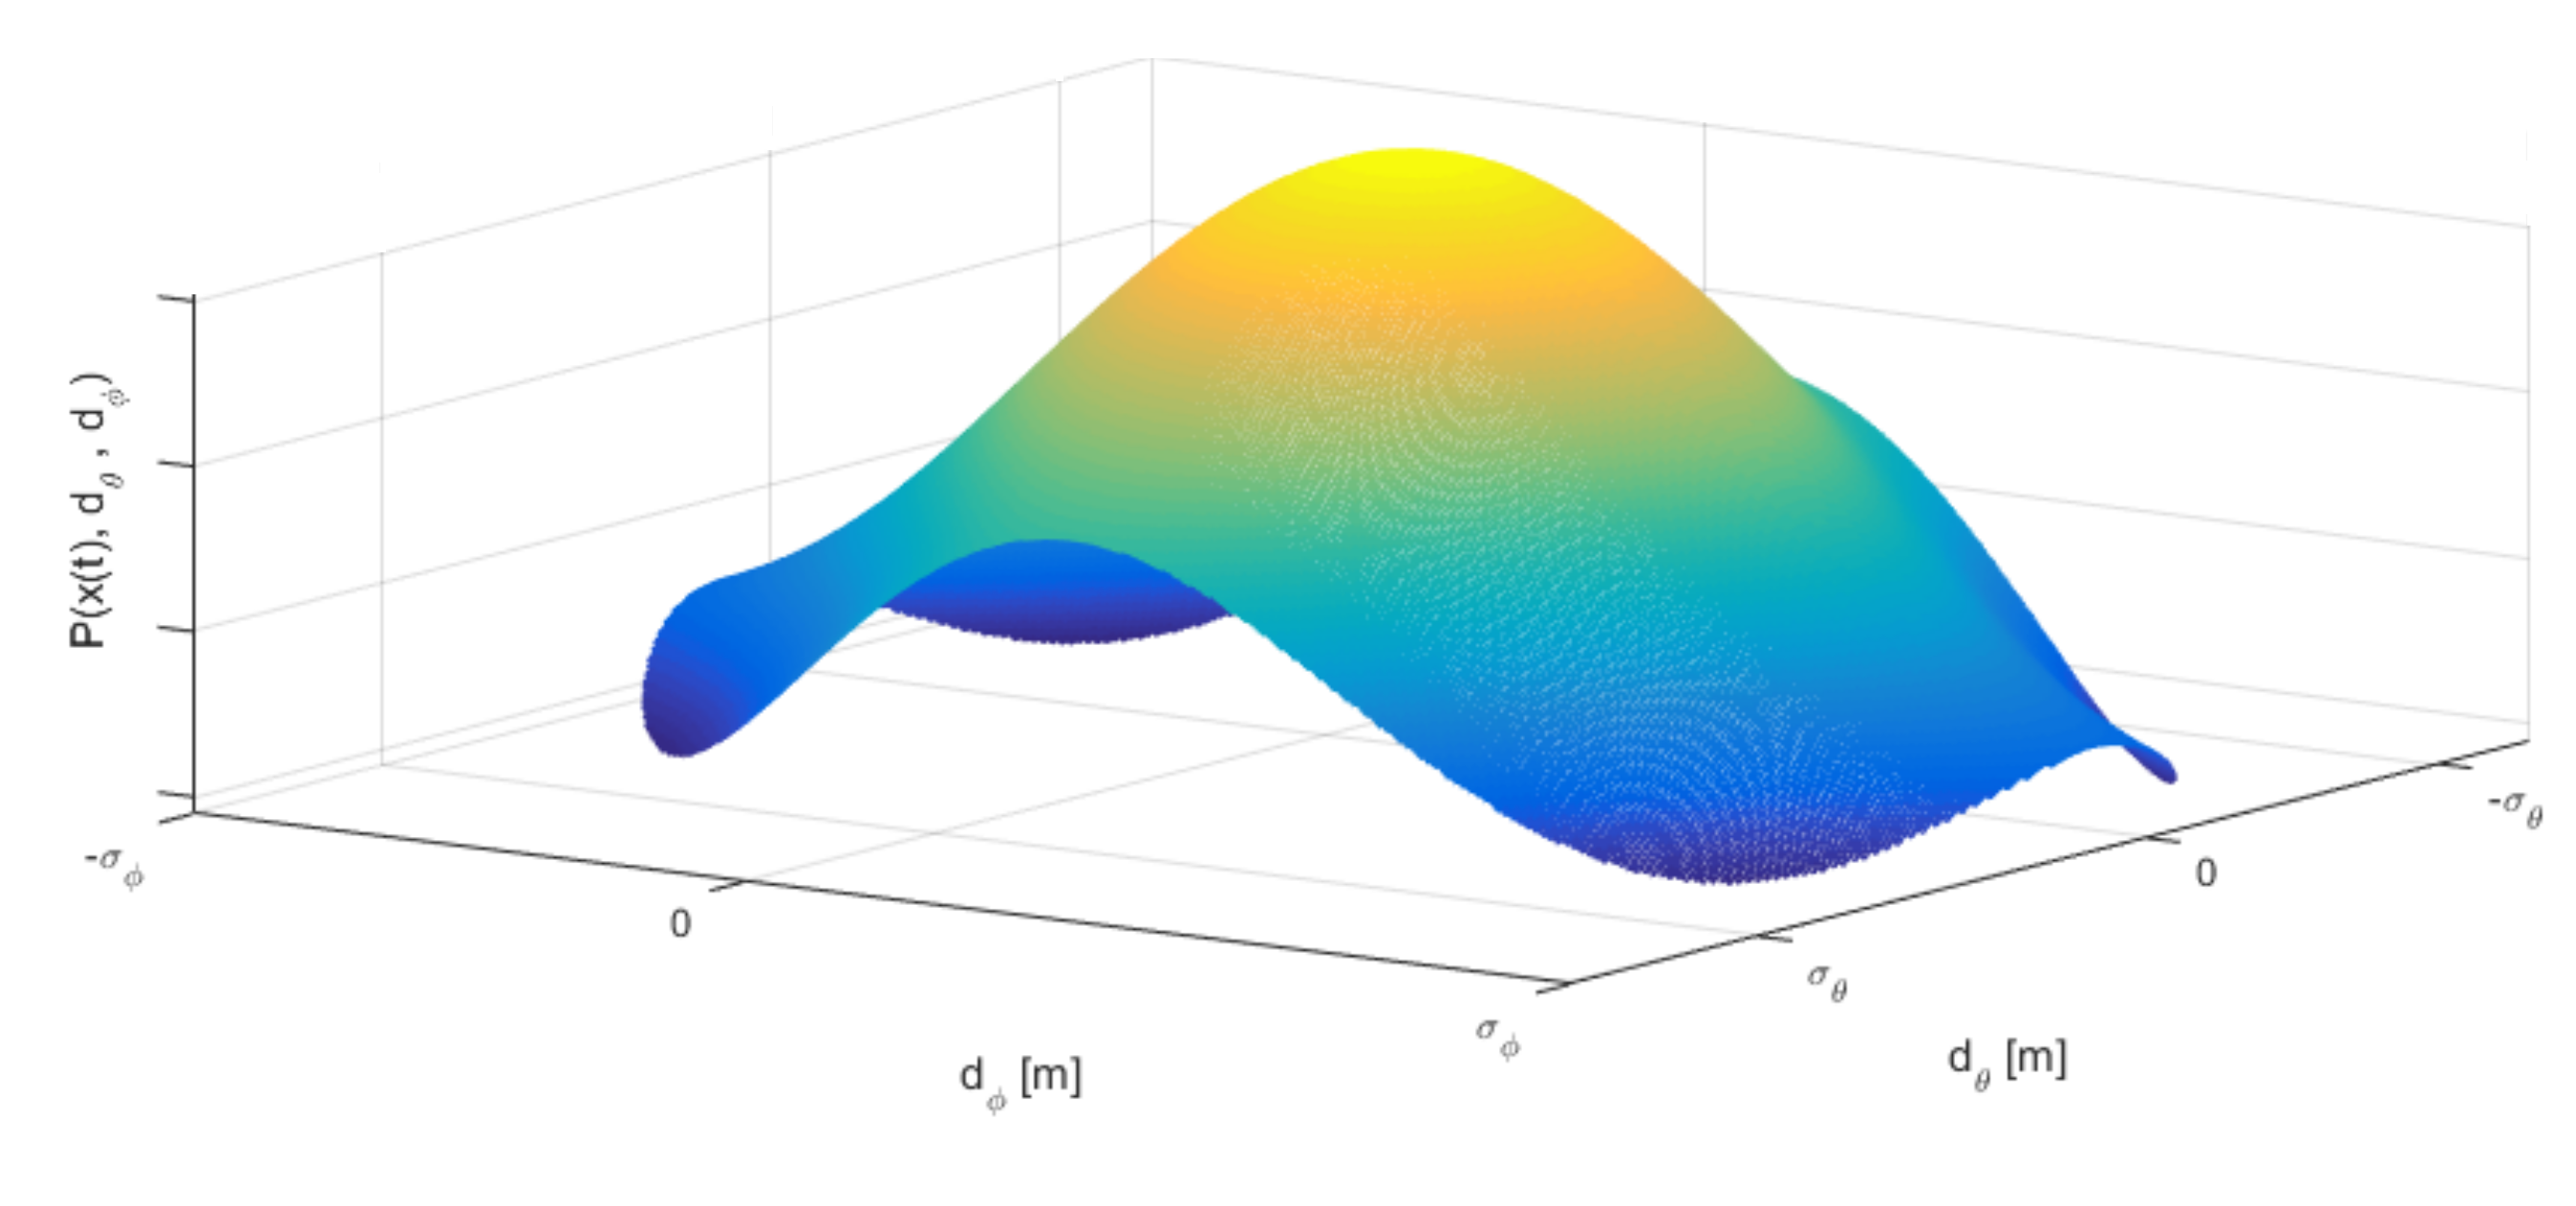
\includegraphics[width=0.9\linewidth]{\FIGDIR/TE015ProbabilisticDistributionOfEllipsoidCutSideForTE016}
            \caption{Intruder passing probability.}
            \label{fig:intruderPassingProbability}
        \end{subfigure}
        \begin{subfigure}{0.48\textwidth}
            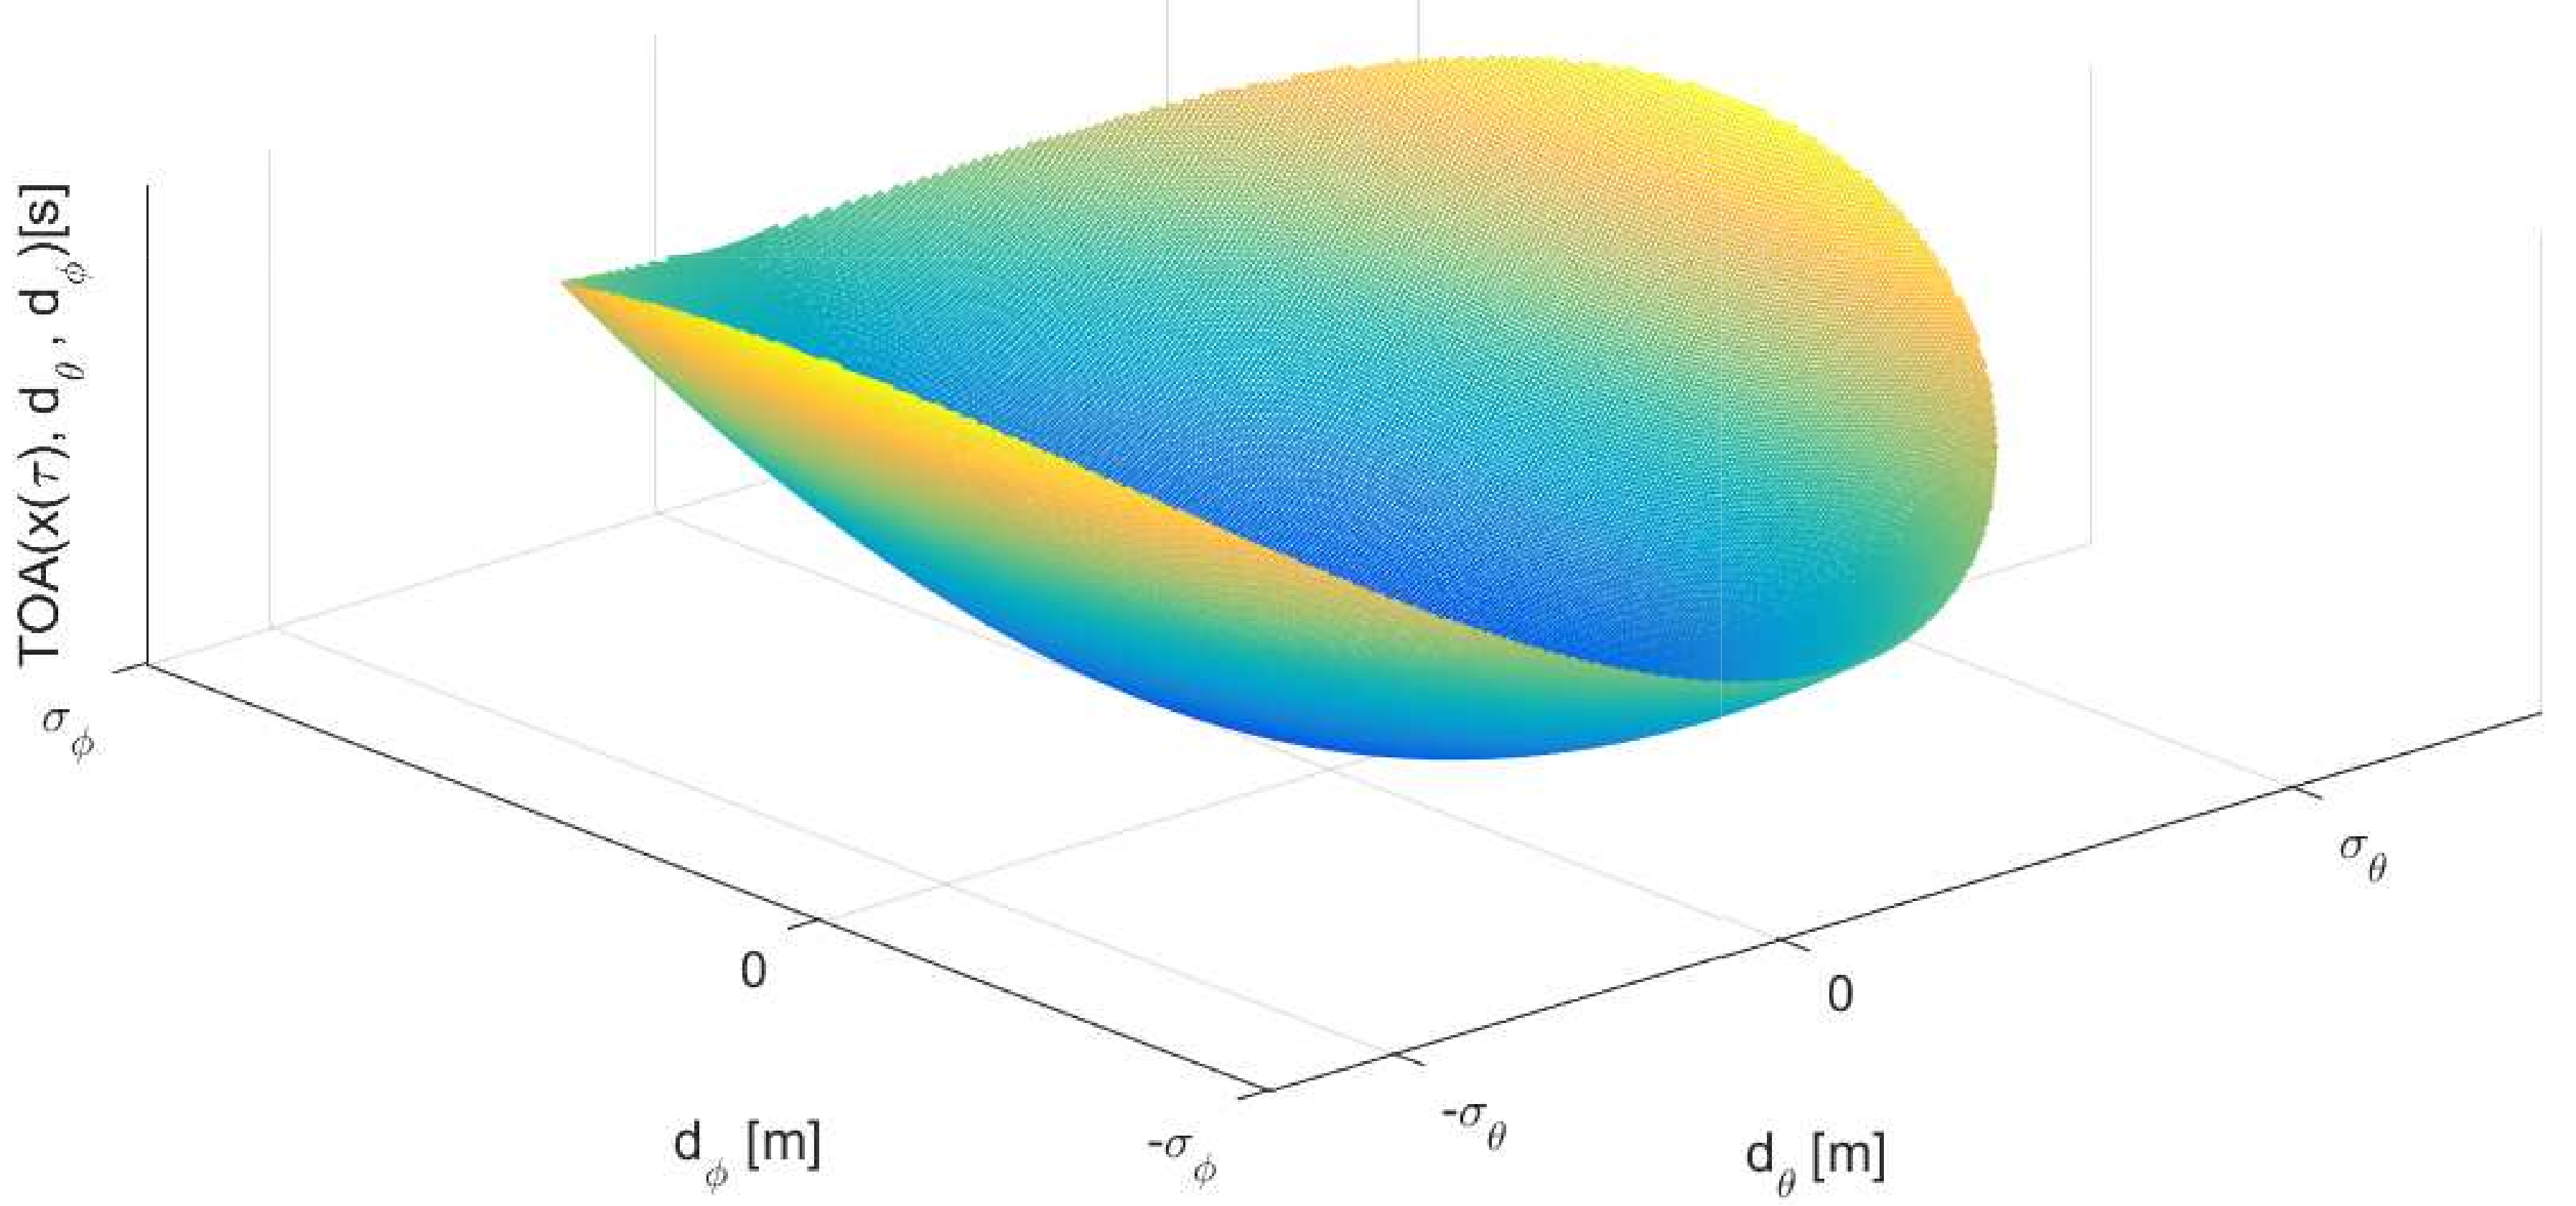
\includegraphics[width=0.9\linewidth]{\FIGDIR/TE016EllipsoidCutTimeOfArrival} 
            \caption{Time of arrival.}
            \label{fig:intruderTimeOfArrival}
        \end{subfigure}
        \caption{Properties for one elliptic cone slice. }
        \label{fig:propertiesEllipticConeSlice}
    \end{figure}

